\begin{frame}{Example: Loop Freedom}
    \begin{center}
        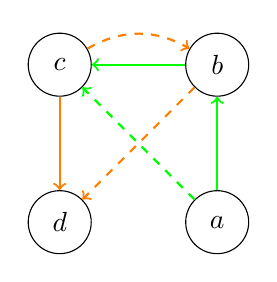
\begin{tikzpicture}[node distance={20mm},main/.style = {draw, circle,minimum size=8mm}]
            \node[main] (a)  {$a$};
            \node[main] (b) [above of=a]  {$b$};
            \node[main] (c) [left of=b] {$c$};
            \node[main] (d)  [below of=c] {$d$};
            \draw [->,green,thick] (a) -- (b);
            \draw [->,green,thick] (b) -- (c);
            \draw [->,orange,thick] (c) -- (d);
            \draw [->,green,thick,dashed] (a) -- (c);
            \draw [->,orange,thick,dashed] (c) edge[bend left] (b);
            \draw [->,orange,thick,dashed] (b) -- (d);
        \end{tikzpicture}
    \end{center}
    \begin{equation*}
        \begin{aligned}
            P           & = p!1                                               \\
            Q           & = q!1                                               \\
            N           & = F \oplus p?1;N_p \oplus q?1;N_q                   \\
            N_p         & = F_p \oplus q?1;F                                  \\
            N_q         & = F_q \oplus p?1;F                                  \\
            SDN         & = \delta_{\mathcal{L}}(N \parallel P \parallel Q) \\
            \mathcal{L} & = \s{p!1,p?1,q!1,q?1}
        \end{aligned}
        \qquad \qquad
        \begin{aligned}
            F    = & ab \oplus ac \oplus ad               \\
                   & \oplus bc \oplus bd \oplus cd        \\
            F_p  = & ac \oplus ad \oplus cd              \\
            F_q  = & ab \oplus ac \oplus ad               \\
                   & \oplus bc \oplus bb \oplus bd        \\
                   & \oplus        cb \oplus cc \oplus cd 
        \end{aligned}
    \end{equation*}
\end{frame}

\begin{frame}{Example: Loop Freedom}
    Property: Loop Freedom
    \begin{align*}
        \f{PV} & = \bigvee_{c \in C} c \in \mathcal{F}(ES(\vec v)) \\
        C      & = \s{c \subset E | \exists e \in c.
            l(e) = bb \vee l(e) = cc }
    \end{align*}
    We can define $M(\s{p_2},q_2) = \F$ as a cause.

    Setting $M(\s{p_2},q_2)$ to true results in $EN(\e,q_2)$ become false
    neither $\s{q_2,bb}$ nor $\s{q_2,cc}$ are not configurations anymore
    We define:
    \begin{center}
        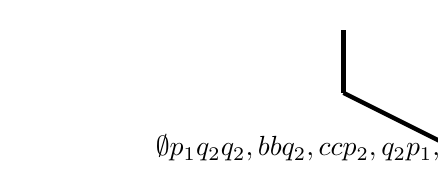
\begin{tikzpicture}[scale=0.8]
            \crd{0}{0}{$\emptyset$}
            \crd[below]{-2}{1}{$\s{p_1}$}
            \crd[below]{2}{1}{$\s{q_2}$}
            \crd[above]{2}{2}{$\s{q_2,bb}$}
            \crd[above]{4}{2}{$\s{q_2,cc}$}
            \crd[above]{0}{2}{$\s{p_2,q_2}$}
            \crd[left]{-2}{2}{$\s{p_1,q_1}$}
            \draw [ultra thick] (0,0) -- (2,1);
            \draw [ultra thick] (0,0) -- (-2,1);
            \draw [ultra thick] (2,1) -- (0,2);
            \draw [ultra thick] (2,1) -- (2,2);
            \draw [ultra thick] (2,1) -- (4,2);
            \draw [ultra thick] (-2,1) -- (-2,2);
        \end{tikzpicture}
    \end{center}
\end{frame}